% Thesis chapter. Standalone-compilable; to drop into a thesis, keep the body and
% discard the preamble. Requires: amsmath amssymb amsthm booktabs graphicx algorithm
% algpseudocode listings xcolor caption.
%
% The results table is GENERATED: paper/results_table.tex is written by
% experiments/paper_assets.py from the run pickles. No number below is transcribed.

\documentclass[11pt]{report}
\usepackage[margin=1.1in]{geometry}
\usepackage{amsmath,amssymb,amsthm,booktabs,graphicx,microtype}
\usepackage{algorithm,algpseudocode}
\usepackage[T1]{fontenc}
\usepackage{xcolor,listings}
\usepackage[font=small,labelfont=bf]{caption}
\usepackage{hyperref}
\hypersetup{colorlinks=true,allcolors=blue!55!black}

\theoremstyle{plain}
\newtheorem{proposition}{Proposition}[chapter]
\newtheorem{theorem}[proposition]{Theorem}
\theoremstyle{definition}
\newtheorem{definition}[proposition]{Definition}
\theoremstyle{remark}
\newtheorem{remark}[proposition]{Remark}

\lstset{basicstyle=\ttfamily\scriptsize, keywordstyle=\color{blue!60!black},
        commentstyle=\color{black!45}\itshape, stringstyle=\color{green!40!black},
        numbers=left, numberstyle=\tiny\color{black!35}, frame=leftline,
        framesep=6pt, rulecolor=\color{black!20}, xleftmargin=14pt,
        breaklines=true, showstringspaces=false, language=Python}

% GENERATED by experiments/paper_assets.py. Do not edit.
\newcommand{\numCovPlain}{0.74}
\newcommand{\numCovStall}{0.81}
\newcommand{\numLossPlain}{0.0619}
\newcommand{\numLossStall}{0.0206}
\newcommand{\numMaeThreshold}{1.56}
\newcommand{\numOverPerfuseEight}{15.3}
\newcommand{\numOverPerfuseFour}{13.3}
\newcommand{\numSlopeThreshold}{0.29}


\begin{document}
\chapter{Metabolically constrained attention}

\section{Motivation}

\subsection{Verification is a search problem before it is a scientific one}

A transformer layer with $H$ attention heads presents an analyst with $2^H$ subsets of
heads and $\binom{H}{2}$ pairwise interactions. At the $H = 32$ used throughout this
chapter that is four billion subsets and 496 pairs. Mechanistic interpretability, which
asks what a network computes and how, therefore begins with a reduction: find a small
subnetwork that does the work, and analyse that instead.

The standard reduction is pruning. One assigns each head an importance score, keeps the
top $k$, and bounds the resulting damage. The scores differ in their ingredients: weight
magnitude, the gradient of the loss with respect to a head gate \cite{michel2019}, the
entropy of the attention distribution \cite{zhai2023}, or a gate learned under an $L_0$
penalty \cite{voita2019}. Two properties are common to all of them, and both are
limiting.

First, \textbf{every score is computed per head, independently}. Head $h$'s importance
does not depend on what the other heads are doing. This is convenient and it is also
false to the situation: heads in a trained transformer are substitutable, and the
literature's own findings reflect this. Randomly chosen subnetworks often retain accuracy
as well as carefully scored ones, which is the weak-link result that the pruning
community has reported repeatedly.

Second, \textbf{the analyst supplies $k$}. The reduction answers ``which $k$ heads'' but
never ``how many''. For interpretability this is exactly backwards. The interesting
quantity is the size of the circuit the task actually requires, and a method that takes
that size as input cannot discover it.

\subsection{What tissue does instead}

Biological neural tissue does not prune on a timescale relevant to inference. It
\emph{allocates}. Cerebral blood flow is approximately conserved: total perfusion is held
near constant by autoregulation, so a local increase is paid for by a decrease elsewhere,
a phenomenon known as vascular steal. The allocation is not a ranking. It is the fixed
point of a feedback loop in which metabolic byproducts accumulate where supply falls short
of demand and act as vasodilators, opening the vessels that serve the shortfall.

Three features of that arrangement are worth transplanting, and it is important to be
precise about which.

\begin{enumerate}
\item \textbf{Conservation.} Supply is redistributed, never destroyed. Starving one
      consumer makes its neighbours richer. This makes the mechanism structurally unlike
      pruning, where removed capacity is simply gone.
\item \textbf{Feedback on a deficit.} The operating point is set by how badly the system
      is performing, not by a threshold chosen in advance.
\item \textbf{Asymmetry between dilation and constriction.} Vasodilators must
      \emph{accumulate}, so a transient shortfall does not open a vessel while a
      sustained one does.
\end{enumerate}

\subsection{What is not being claimed}
\label{sec:notclaimed}

Kozachkov, Kastanenka and Krotov \cite{kozachkov2023} show that a neuron--astrocyte
network can implement the core computation of a transformer, with the astrocyte supplying
the normalisation in self-attention. Their construction is used in
Section~\ref{sec:algebra} as a point of algebraic comparison, because the astrocytic gain
is a conserved divisive field of the same form as the supply field defined here. That
comparison is an identity of \emph{form} and nothing more. Their work establishes a
plausible substrate for normalisation; it does not model, measure, or test metabolic
gating, and their gain is a function of presynaptic drive rather than of blood supply.
No biological support for the mechanism studied here is drawn from it. The physiological
question of whether attention in tissue is metabolically gated is untouched by anything
in this chapter.

\section{A conserved supply field}
\label{sec:algebra}

\subsection{The layer as one product}

Following the matrix conventions of \cite{kozachkov2023}, let
$X \in \mathbb{R}^{d \times N}$ hold $N$ token embeddings of dimension $d$ and let
$Y$ hold the memory the layer attends to. Head $h \in [H]$ computes
\begin{equation}
  Q_h = W_Q^{(h)} X, \quad K_h = W_K^{(h)} Y, \quad V_h = W_V^{(h)} Y,
  \quad A_h = \operatorname{softmax}\!\Bigl(\tfrac{Q_h^\top K_h}{\sqrt{d_k}}\Bigr),
\end{equation}
with per-head output $O_h = V_h A_h^\top \in \mathbb{R}^{d_k \times N}$. Write
$W_O^{(h)} \in \mathbb{R}^{d_{\text{out}} \times d_k}$ for the $h$-th column block of the
output projection and stack the head outputs into
$O = [O_1^\top \cdots O_H^\top]^\top \in \mathbb{R}^{H d_k \times N}$.

\begin{definition}[Conserved supply]
\label{def:supply}
A \emph{supply rule} maps a demand vector $d \in \mathbb{R}^H$ to a gain vector
$g = \mathcal{S}(d) \in \mathbb{R}_{\ge 0}^H$ subject to
\begin{equation}
  \label{eq:cons}
  \textstyle\sum_{h} g_h = H .
\end{equation}
With $G = \operatorname{diag}(g)$ the gated layer is the single product
\begin{equation}
  \label{eq:kron}
  \boxed{\;\mathcal{T}_g(X) \;=\; W_O \,\bigl(G \otimes I_{d_k}\bigr)\, O,
  \qquad \operatorname{tr} G = H .\;}
\end{equation}
\end{definition}

Equation~\eqref{eq:kron} is the whole construction. Conservation is a trace constraint;
the dense layer is the special case $G = I_H$; and the Kronecker factor $I_{d_k}$ records
that supply is allocated per head rather than per coordinate. Every rule studied here is
of the form
\begin{equation}
  \label{eq:equalshare}
  g \;=\; \tfrac{H}{B}\,\mathbf{1}_S, \qquad S \subseteq [H],\; S \neq \emptyset,\;
  B = |S|,
\end{equation}
an equal share among a \emph{perfused set} $S$, with $G = (H/B) P_S$ for the diagonal
projector $P_S$. The rules differ only in how $S$ is chosen from $d$, and $B$ is never
supplied as an argument.

\subsection{Why the surviving circuit is the whole circuit}

\begin{proposition}[Exact reduction]
\label{prop:reduction}
Let $g$ be as in \eqref{eq:equalshare} with zero leak. Then
\begin{equation}
  \mathcal{T}_g(X)
  \;=\; \tfrac{H}{B}\, W_O (P_S \otimes I_{d_k}) O
  \;=\; \widetilde{W}_{O,S}\, O_S,
  \qquad \widetilde{W}_{O}^{(h)} = \tfrac{H}{B} W_O^{(h)},
\end{equation}
so $\mathcal{T}_g$ \emph{is} a $B$-head layer, and $\operatorname{rank}\mathcal{T}_g \le
B\,d_k$. Furthermore $\partial\mathcal{T}_g/\partial\theta_h = 0$ for every parameter
$\theta_h$ of a head $h \notin S$.
\end{proposition}

\begin{proof}
$P_S$ annihilates every term with $h \notin S$ and the scalar $H/B$ is absorbed into
$W_O^{(h)}$, leaving \eqref{eq:kron} with $H$ replaced by $B$. The rank bound follows
since the image is a sum of $B$ subspaces of dimension at most $d_k$. For the gradient,
$\mathcal{T}_g$ depends on $\theta_h$ only through the product $g_h W_O^{(h)} O_h$ and
$g_h = 0$.
\end{proof}

This proposition is the reason the construction is worth the trouble. A pruning paper owes
its reader an argument about what the removed heads were contributing; here there is
nothing to argue, because the reduction is an identity rather than an approximation, and
starved heads receive no gradient so nothing can hide in them. At $H = 32$, $B = 4$ an
analyst faces $8\times$ fewer single-head hypotheses and $83\times$ fewer pairwise ones,
exactly and with no residual term to bound.

\subsection{Relation to astrocytic normalisation}

In \cite{kozachkov2023} the reading phase of the neuron--astrocyte circuit computes
\begin{equation}
  \ell_t = \tfrac{1}{p}\,H\varphi(q_t) + x_t,
  \qquad p = \tfrac{1}{m}\textstyle\sum_{j} \varphi(k_j)^\top \varphi(q_t),
\end{equation}
where spatial averaging of astrocyte processes makes the modulation
$\widetilde P_{i\ell} = 1/p$ a \emph{single scalar gain shared across the astrocyte's
domain}, and $p$ is the reciprocal of pooled presynaptic drive. That is a conserved
divisive gain field of exactly the type in Definition~\ref{def:supply}, on a different
index set: theirs runs over the synapses of one domain with the softmax partition
function conserved, ours over attention heads with total flow conserved. Writing
$\beta \in [0,1]$ for the degree to which demand is pooled within a neighbourhood, their
construction is the fully pooled endpoint $\beta = 1$. Section~\ref{sec:notclaimed}
states the limits of this correspondence.

\section{A benchmark whose circuit is known}
\label{sec:bench}

\begin{figure}[t]
  \centering
  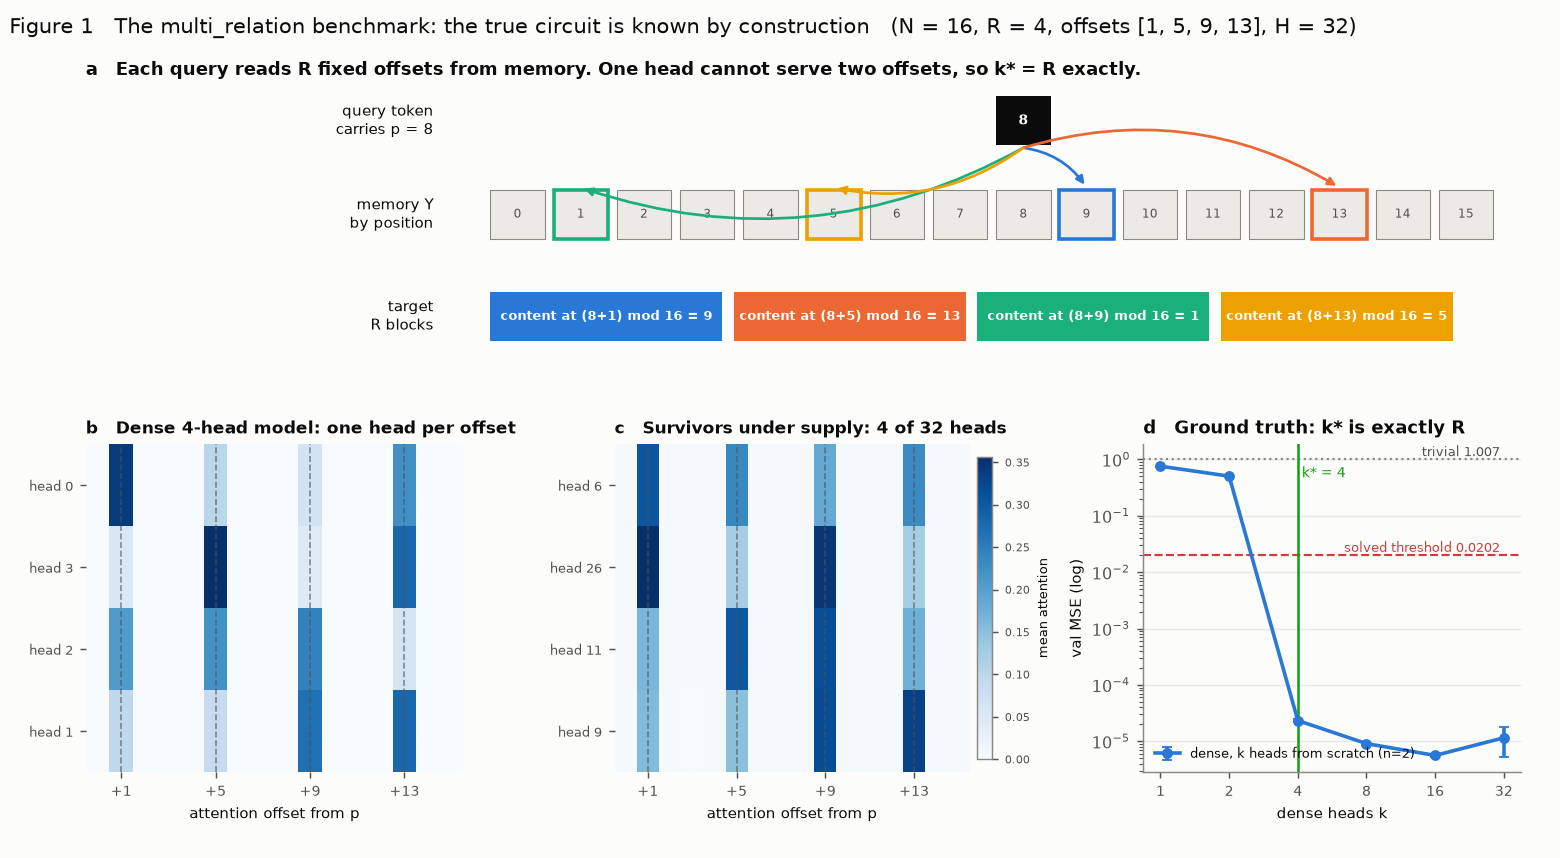
\includegraphics[width=\textwidth]{../figures/fig1_task.png}
  \caption{\textbf{The \texttt{multi\_relation} benchmark.} (a) Each query token carries a
  position $p$ and must emit the content stored at $R$ fixed offsets from it. (b) The
  measured attention-offset profile of a dense $R$-head model: one head per offset,
  recovering exactly the true set $\{1,5,9,13\}$. (c) The heads that survive under
  conserved supply, scored at the gate the run converged to. (d) Dense models trained from
  scratch at each head count; the loss crosses the solved threshold exactly at
  $k^\star = R$. Panels (b)--(d) are measurements, not illustrations.}
  \label{fig:task}
\end{figure}

Any claim about discovering circuit size needs a task whose circuit size is known. We use
\texttt{multi\_relation} (Figure~\ref{fig:task}). Each query token carries a key position
$p \in \{0,\dots,N-1\}$. The target is $R$ concatenated blocks, block $r$ holding the
content stored at position $(p + \delta_r) \bmod N$ for a fixed offset set
$\{\delta_r\}_{r=1}^R$.

\begin{remark}[Why $k^\star = R$ exactly]
A single head implements one query--key geometry. Because $W_Q$ is linear, the geometry
required to attend from $p$ to $p + \delta$ differs for each $\delta$, so one head cannot
serve two offsets. The minimum head count is therefore $R$, set by \emph{function} rather
than by capacity, and every head in a minimal circuit has a name: the offset it
implements.
\end{remark}

This is what allows interpretability to be scored directly. We define \emph{role coverage}
as the fraction of true offsets implemented by some perfused head, where a head's role is
the offset at which its mean attention profile peaks. Existing pruning work reports
accuracy retention instead, because no standard benchmark has known head roles. Training
dense models from scratch at each head count confirms $k^\star = R$ at every $R$ tested
(Figure~\ref{fig:task}d).

\section{Supply mechanisms}

\subsection{Fixed-quantile supply, and why it cannot work}

The natural rule perfuses heads whose standardised demand exceeds $\kappa$ standard
deviations (Algorithm~\ref{alg:thresh}). It fails, and not for want of tuning.

\begin{algorithm}[t]
\caption{Fixed-quantile supply}
\label{alg:thresh}
\begin{algorithmic}[1]
\Require demand $d \in \mathbb{R}^H$ (standardised), threshold $\kappa$, total $H$
\State $\theta \gets \operatorname{mean}(d) + \kappa \cdot \operatorname{std}(d)$
\State $S \gets \{h : d_h > \theta\}$
\If{$S = \emptyset$} \State $S \gets \{\arg\max_h d_h\}$
  \Comment{never fully infarct} \EndIf
\State \Return $g$ with $g_h = H/|S|$ for $h \in S$, else $0$
\end{algorithmic}
\end{algorithm}

\begin{theorem}[Fixed-quantile rules cannot track $k^\star$]
\label{thm:impossible}
Let $d$ be standardised and let $F_d$ be its empirical distribution function. Then the
perfused count produced by Algorithm~\ref{alg:thresh} is
\begin{equation}
  \label{eq:quantile}
  B \;=\; H\bigl(1 - F_d(\kappa)\bigr),
\end{equation}
a functional of $(\kappa, H)$ and the \emph{shape} of $F_d$ alone. Consequently
$\mathrm{d}B/\mathrm{d}k^\star = -H\,\partial_{k^\star} F_d(\kappa)$, and tracking
requires the demand distribution to deform at exactly the rate $-1/H$ at the operating
point. No property of the rule can enforce this, because the rule observes nothing that
depends on $k^\star$.
\end{theorem}

\begin{proof}
The number of coordinates exceeding $\kappa$ is $H(1-F_d(\kappa))$ by definition of
$F_d$. Standardisation fixes the first two moments, so $B$ depends on $d$ only through
its shape. Differentiating in $k^\star$ gives the second claim.
\end{proof}

The content of Theorem~\ref{thm:impossible} is that standardisation removes the only two
moments that could carry information about the task, leaving a question about the shape of
a distribution that the architecture, not the task, fixes.

\subsection{Autoregulated supply}

Theorem~\ref{thm:impossible} indicates the repair: the operating point must be set by a
quantity that depends on task difficulty. We close the loop on a metabolic deficit.

\begin{definition}[Autoregulated supply]
\label{def:autoreg}
Fix a target loss $L^\star$, taken as a fraction of the trivial (predict-the-mean)
baseline so that it is scale-free across tasks. The threshold becomes a state variable,
\begin{equation}
  \label{eq:loop}
  \kappa_{t+1} \;=\; \Pi_{[\kappa_-,\kappa_+]}\!\bigl(\kappa_t + \eta\,\phi_t\,e_t\bigr),
  \qquad e_t = \log L^\star - \log \widehat L_t ,
\end{equation}
with $\Pi$ the projection onto the admissible interval. The error is a log ratio, so the
loop is invariant to the scale of the loss. Plain autoregulation takes $\phi_t \equiv 1$.
\end{definition}

Let $L_\infty(B)$ denote the loss the model converges to when held at $B$ perfused heads.
Because the head count is an integer, $\{L_\infty(B)\}$ is a staircase.

\begin{theorem}[The loop selects the minimal sufficient circuit]
\label{thm:autoreg}
If $L_\infty$ is nonincreasing in $B$ and $B$ is nonincreasing in $\kappa$, then every
interior fixed point of \eqref{eq:loop} driven by $L_\infty$ satisfies
$\widehat L = L^\star$ and selects
\begin{equation}
  B^\star(L^\star) \;=\; \min\{B : L_\infty(B) \le L^\star\}.
\end{equation}
If $L_\infty(k^\star) < L^\star < L_\infty(k^\star - 1)$ then $B^\star = k^\star$, and
this holds for \emph{every} $L^\star$ in that interval.
\end{theorem}

The width of that interval is a property of the benchmark. On \texttt{multi\_relation} at
$R = 4$ the measured staircase is $L_\infty(1) = 0.755$, $L_\infty(2) = 0.503$,
$L_\infty(4) = 2\times 10^{-5}$ against a trivial baseline of $1.007$, so the admissible
interval spans roughly four orders of magnitude. This is what distinguishes
Theorem~\ref{thm:autoreg} from the fixed-$\kappa$ rule, whose working setting was a single
point.

\subsection{The specification failure, and the stall gate}

Equation~\eqref{eq:loop} is driven by the \emph{instantaneous} loss $\widehat L_t$,
whereas Theorem~\ref{thm:autoreg} is a statement about $L_\infty(B)$. Early in training
$\widehat L_t \gg L_\infty(B)$ for every $B$, so $e_t < 0$ persistently and
\begin{equation}
  \kappa_t \approx \kappa_0 - \eta\textstyle\sum_{s<t}|e_s| \;\longrightarrow\; \kappa_-,
\end{equation}
driving $B \to H$ before the learner has revealed what $B$ was sufficient. This is a
\emph{specification} failure rather than a tuning failure: the loop controls the wrong
quantity. Measured, a target four times tighter than the working one drove $B$ to
\numOverPerfuseFour{} where $4$ sufficed and to \numOverPerfuseEight{} where $8$ did.

In tissue the vasodilatory signal is an accumulated byproduct, so dilation requires the
shortfall to persist. Let $\bar L_t$ be a slower average of the loss than $\widehat L_t$
and let $\rho_t = (\bar L_t - \widehat L_t)/\bar L_t$ be the relative improvement rate.

\begin{algorithm}[t]
\caption{Stall-gated autoregulation (one training step)}
\label{alg:stall}
\begin{algorithmic}[1]
\Require state $\kappa$, target $L^\star$, gain $\eta$, stall threshold $\varepsilon$
\State $\widehat L \gets$ minibatch loss; \; update slow average $\bar L$
\State $e \gets \log L^\star - \log \widehat L$
\State $\rho \gets (\bar L - \widehat L)/\bar L$ \Comment{$>0$ while still descending}
\If{$e < 0$ \textbf{and} $\rho > \varepsilon$}
  \State \textbf{return} $\kappa$ \Comment{acute deficit: hold, do not dilate}
\EndIf
\State $\kappa \gets \Pi(\kappa + \eta\,\mathrm{clip}(e,\pm 4))$
  \Comment{constriction is never gated}
\State \textbf{return} $\kappa$
\end{algorithmic}
\end{algorithm}

\begin{proposition}[The gate restores the theorem's hypothesis]
\label{prop:stall}
Under Algorithm~\ref{alg:stall}, every dilation step occurs at a time with
$\rho_t \le \varepsilon$, hence
$\widehat L_t = L_\infty(B_t)\bigl(1 + O(\varepsilon)\bigr)$ and
\begin{equation}
  e_t \;=\; \log L^\star - \log L_\infty(B_t) \;+\; O(\varepsilon).
\end{equation}
To first order in $\varepsilon$ the gated loop is \eqref{eq:loop} driven by the converged
loss, and its fixed points are those of Theorem~\ref{thm:autoreg}.
\end{proposition}

\begin{proof}
By construction $\phi_t = 0$ whenever $e_t < 0$ and $\rho_t > \varepsilon$, so every step
that decreases $\kappa$ has $\rho_t \le \varepsilon$. Since $\rho_t$ measures the relative
descent of $\widehat L$ toward its limit, $\rho_t \le \varepsilon$ gives
$\widehat L_t = L_\infty(B_t)(1 + O(\varepsilon))$, and the logarithm converts the
multiplicative error into an additive one.
\end{proof}

\begin{remark}[Two timescales, enforced rather than hoped for]
Proposition~\ref{prop:stall} is a separation-of-timescales argument. The plain loop attains
the same separation only by taking $\eta$ small enough to be slower than the learner
everywhere, which asks one global constant to respect a rate that varies across training.
The gate enforces the separation adaptively, waiting exactly as long as the learner needs
at each point. The control that distinguishes these is plain autoregulation at $\eta/10$:
if sluggishness alone sufficed, that arm would match the gated one.
\end{remark}

\section{Implementation}

The code is organised so that the two axes of the design, what is sensed and how it is
allocated, can be varied independently. Listing~\ref{lst:gate} gives the supply rules and
Listing~\ref{lst:loop} the controller.

\begin{lstlisting}[caption={Conserved allocation. Every rule routes through
\texttt{\_from\_active}, so conservation is structural rather than a property each rule
must remember.}, label={lst:gate}]
def _from_active(self, d, active, total):
    """Equal share among the perfused set, leak to the rest. Conserves sum(gate)."""
    if active.sum() == 0:                       # never fully infarct
        active = torch.zeros_like(d, dtype=torch.bool)
        active[d.argmax()] = True
    g = torch.full_like(d, self.leak)
    g[active] = (total - self.leak * (~active).sum()) / active.sum()
    return g

def gate_threshold(self, d, kappa, total=None):
    """theta = mean + kappa*std. The perfused set, and therefore B, emerges."""
    total = total if total is not None else self.H
    theta = d.mean() + kappa * d.std().clamp_min(1e-6)
    return self._from_active(d, d > theta, total)
\end{lstlisting}

\begin{lstlisting}[caption={The controller. \texttt{stall\_gate} $> 0$ enables
Algorithm~\ref{alg:stall}; with \texttt{loss\_ema} $=0$ and \texttt{autoreg\_every} $=1$
the sensed loss is the raw minibatch loss.}, label={lst:loop}]
def autoregulate(self, loss, target, step=0):
    l = float(loss)
    sensed = l if self.loss_ema_c == 0.0 else self._debiased_ema(l, step)
    self.slow_loss.mul_(self.slow_c).add_((1 - self.slow_c) * l)
    if step % self.autoreg_every:
        return float(self.kappa_state)
    err = math.log(max(target, 1e-12)) - math.log(max(sensed, 1e-12))
    if self.stall_gate > 0.0 and err < 0.0:
        slow = float(self.slow_loss) / (1 - self.slow_c ** max(1, step + 1))
        rate = (slow - sensed) / max(slow, 1e-12)     # > 0 while still improving
        if rate > self.stall_gate:
            return float(self.kappa_state)            # acute: hold
    self.kappa_state += self.autoreg_gain * max(-4.0, min(4.0, err))
    self.kappa_state.clamp_(self.kappa_floor, self.kappa_ceil)
    return float(self.kappa_state)
\end{lstlisting}

\paragraph{Conservation as a tested invariant.}
Equation~\eqref{eq:cons} is not documentation but an assertion in the test suite, executed
for every supply rule:
\begin{lstlisting}[numbers=none]
for supply in ["topk", "threshold", "territory", "gap", "otsu",
               "autoreg", "poiseuille", "watershed", "watershed_auto"]:
    g = HemoAttn(replace(cfg, supply=supply)).gate(kappa=1.0, B_active=3)
    assert abs(float(g.sum()) - m.H) < 1e-3
\end{lstlisting}

\paragraph{Measurement conventions.}
Three conventions are load-bearing and each was adopted after a measurement error.
\emph{(i)} Head ablation is always performed at full perfusion; run at a starved gate,
most heads sit at zero and every rank correlation becomes a tie artefact. \emph{(ii)}
Thresholds separating ``solved'' from ``unsolved'' are a fraction of the dense-to-trivial
\emph{gap}, never of the dense loss alone, which becomes unreachable once a task is solved
exactly. \emph{(iii)} For mechanisms in which $B$ emerges, the reported $B$ is the median
over the held phase rather than the final step, since a closed loop's final gate is one
sample of its trajectory.

\section{Results}

\begin{table}[t]
  \centering\small
  % GENERATED by experiments/paper_assets.py. Do not edit.
\begin{tabular}{@{}lccccc@{}}
\toprule
& $\mathrm{d}B/\mathrm{d}k^\star$ & MAE & role & val &  \\
supply rule & (ideal $1.00$) & (heads) & cov. & MSE & $n$ \\
\midrule
\multicolumn{6}{@{}l}{\emph{closed loop: supply answers to a metabolic deficit}} \\
autoreg & +1.00 & 0.00 & 0.74 & 0.0619 & 3 \\
\textbf{autoreg + stall gate} & +1.00 & 0.00 & 0.81 & 0.0206 & 3 \\
\addlinespace[2pt]
\midrule
\multicolumn{6}{@{}l}{\emph{open loop: supply answers to the demand distribution}} \\
watershed & +0.32 & 7.83 & 0.98 & 0.0003 & 1 \\
fixed threshold & +0.29 & 1.56 & 0.62 & 0.2736 & 3 \\
otsu & -0.07 & 2.40 & 0.69 & 0.2751 & 3 \\
poiseuille $n{=}4$ & -0.26 & 2.50 & 0.58 & 0.4105 & 1 \\
poiseuille $n{=}1$ & -0.57 & 3.75 & 0.61 & 0.3939 & 1 \\
gap & -0.92 & 6.53 & 0.77 & 0.1992 & 3 \\
\bottomrule
\end{tabular}

  \caption{Supply rules on \texttt{multi\_relation} at $H{=}32$, $d_k{=}32$, $N{=}16$,
  grouped by whether supply answers to task performance or only to the demand
  distribution. Slope is fitted over $k^\star \in \{2,\dots,8\}$; MAE is
  $|B - k^\star|$ in heads. Generated from the run pickles by
  \texttt{experiments/paper\_assets.py}.}
  \label{tab:arms}
\end{table}

\begin{figure}[t]
  \centering
  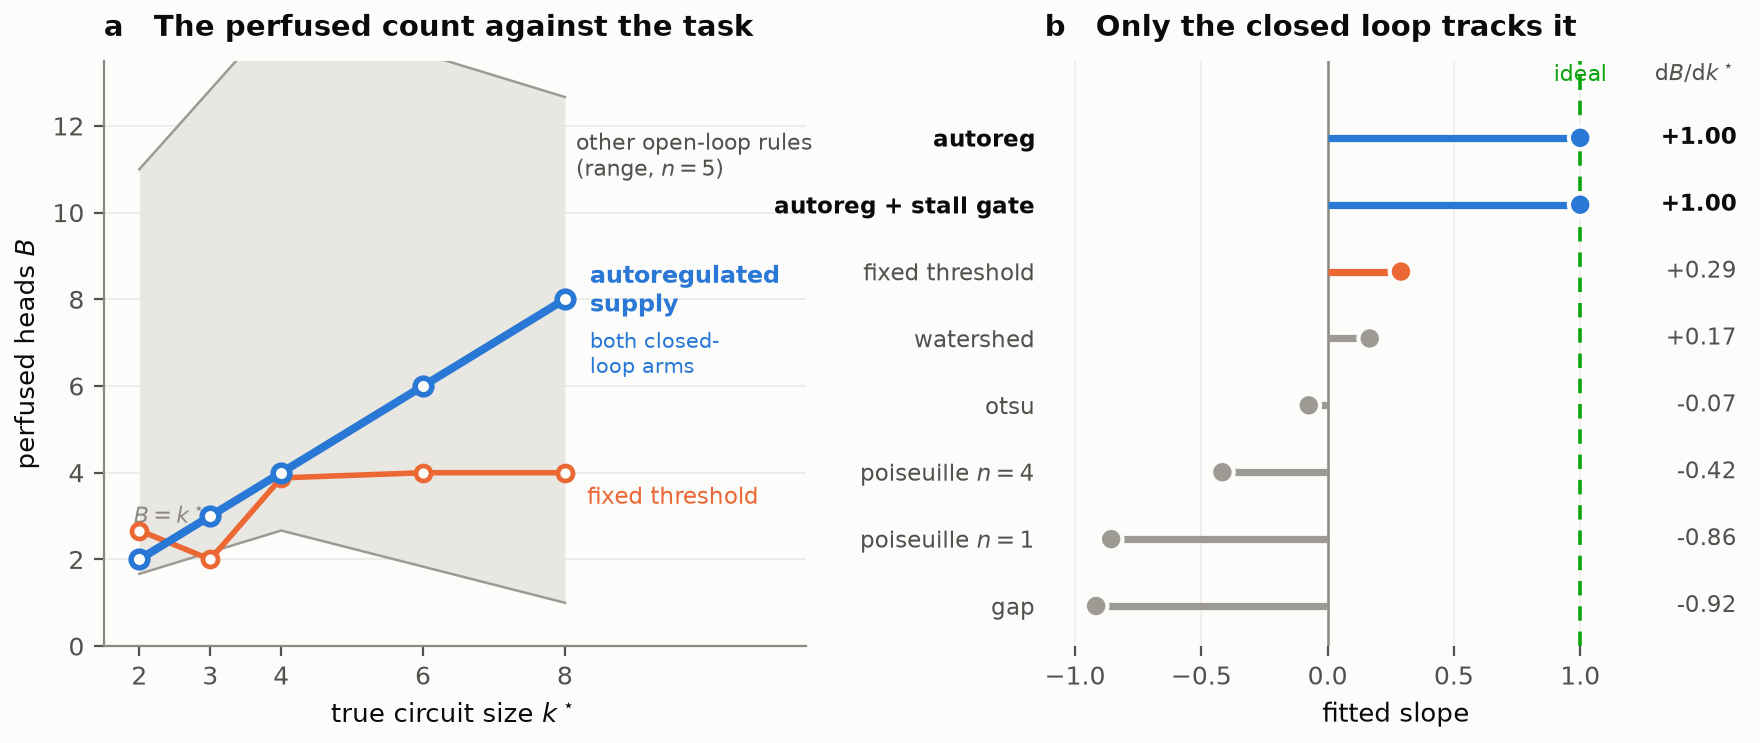
\includegraphics[width=\textwidth]{../figures/fig_arms.png}
  \caption{\textbf{Only the closed loop tracks circuit size.} (a) Perfused count against
  true circuit size. Both autoregulated arms give identical $B$ and are drawn as one line,
  which lies on the identity; the band spans the remaining open-loop rules. (b) Fitted
  $\mathrm{d}B/\mathrm{d}k^\star$ for every arm.}
  \label{fig:arms}
\end{figure}

\subsection{Tracking}

Table~\ref{tab:arms} and Figure~\ref{fig:arms} give the comparison. Both autoregulated
arms achieve $\mathrm{d}B/\mathrm{d}k^\star = 1.00$ at zero mean absolute error. Every
open-loop rule fails and three have \emph{negative} slope.

Poiseuille is the informative failure. Its perfused \emph{set} is identical to the fixed
threshold's by construction, since both cut at $\theta = \operatorname{mean} + \kappa
\operatorname{std}$; only the shares within that set differ, graded as $r^n$ with $r$ the
tone above threshold. It nonetheless scores worse. Selection, not allocation, is the
binding constraint.

\subsection{The control that decides it}

Plain autoregulation tracked $k^\star$ exactly at one loss target. The question is whether
that target is a tuned setting or a working range, and Theorem~\ref{thm:autoreg} predicts
a range spanning the staircase gap.

\begin{table}[h]
\centering\small
% GENERATED by experiments/paper_assets.py. Do not edit.
\begin{tabular}{@{}lccc@{}}
\toprule
& \multicolumn{3}{c}{$B$ at $k^\star = 2,\,4,\,8$} \\
\cmidrule(l){2-4}
loss target & plain autoreg & \; & $+$ stall gate \\
\midrule
$0.005$ & $3.0, 13.3, 15.3$ & & $3.5, 4.0, 8.0$ \\
$0.02$ & $2.0, 4.0, 8.0$ & & $2.0, 4.0, 8.0$ \\
$0.05$ & $2.0, 4.0, 7.0$ & & $2.0, 4.0, 7.0$ \\
\midrule
MAE over the range & $2.07$ heads & & $\mathbf{0.28}$ heads \\
exact & $5/9$ & & $\mathbf{7/9}$ \\
\bottomrule
\end{tabular}

\caption{The target control. At the tight target the plain loop dilates through the early
transient and over-perfuses by an order of magnitude; the gate holds it to the correct
count. Mean absolute error at that target falls from $5.89$ to $0.50$ heads, a factor of
$11.8$. This is the prediction of Proposition~\ref{prop:stall}, tested after it was
derived.}
\label{tab:target}
\end{table}

Table~\ref{tab:target} gives the result. The stall gate converts an order-of-magnitude
failure into an off-by-one error and turns the working band from a point into a range,
which is the difference between a tuned setting and a mechanism. The gate's other effect
is on interpretability rather than on counting: role coverage rises from \numCovPlain{} to \numCovStall{}
and converged loss from \numLossPlain{} to \numLossStall{}, at identical tracking.

\subsection{Negative results}

Four mechanisms produced nulls. They are reported because each rules something out.

\begin{description}\itemsep2pt
\item[Territory compaction.] Territory span tracked the territory count at every setting
  and role coverage declined gently below $T = R$ rather than collapsing. The cause is
  structural: the never-fully-infarct floor was applied per territory, guaranteeing one
  live head per territory, so $B \ge T$ by construction and compaction below $T$ was
  impossible. Additionally, every live territory received an equal share irrespective of
  its demand, so flow never moved between territories and vascular steal, the entire
  motivation for the mechanism, was absent. What ran was $T$ independent models each
  applying Algorithm~\ref{alg:thresh}.
\item[Delay.] A lag $\tau$ between demand and supply produced no optimum: $\tau \in
  \{0,1,5,20\}$ spans $10^{-4}$ in converged loss with overlapping intervals. The
  predicted failure mode at long $\tau$ is absent; perfused-set churn peaks at one change
  per $272$ steps, so there is no oscillation for a longer lag to trade against.
\item[Pooled demand.] Averaging demand within a neighbourhood changed nothing across its
  full range, and full pooling had the worst converged loss of the four settings.
\item[The gating signal is not the best predictor of importance.] Across all runs at full
  perfusion, the demand the mechanism gates on scores $\rho = +0.379$ against ablation
  delta, below both the query norm ($+0.484$) and attention entropy ($+0.452$) on the same
  runs. The mechanism works despite its sensor rather than because of it.
\end{description}

\section{Limitations}

Three limitations bear on how the result should be stated.

First, $\min\{B : L_\infty(B) \le L^\star\}$ is close to the \emph{definition} of the
minimal circuit. The defensible claim is therefore that one run of a feedback loop
recovers what otherwise requires a sweep over $B$ with a full training run at each value.
That is an efficiency result about circuit discovery, not a demonstration that metabolic
constraint reveals circuit size from first principles.

Second, the stall gate introduces $\varepsilon$, and the obvious objection is that a tuned
target has been replaced by a tuned threshold. Proposition~\ref{prop:stall} predicts
otherwise, since $\varepsilon$ enters only as an $O(\varepsilon)$ perturbation of the
control error while $L^\star$ enters the fixed point directly, but that prediction
requires its own control and is not yet settled.

Third, the correct head \emph{count} is weaker than the correct head \emph{roles}. Role
coverage does not reach unity, and at one circuit size the loop selected exactly $k^\star$
heads for a model that had not solved the task. Selection and optimisation are distinct
problems and only the first is addressed here.

\begin{thebibliography}{9}
\bibitem{kozachkov2023} L.~Kozachkov, K.~V.~Kastanenka, D.~Krotov.
  Building transformers from neurons and astrocytes. \emph{PNAS} 120(34):e2219150120, 2023.
\bibitem{michel2019} P.~Michel, O.~Levy, G.~Neubig.
  Are sixteen heads really better than one? \emph{NeurIPS}, 2019.
\bibitem{voita2019} E.~Voita, D.~Talbot, F.~Moiseev, R.~Sennrich, I.~Titov.
  Analyzing multi-head self-attention. \emph{ACL}, 2019.
\bibitem{zhai2023} S.~Zhai et al.
  Stabilizing transformer training by preventing attention entropy collapse. \emph{ICML}, 2023.
\end{thebibliography}

\end{document}
